\documentclass{beamer}
\usepackage[utf8]{inputenc}
\usepackage[ngerman]{babel}
\usepackage{graphicx}
\usetheme{CambridgeUS}
\usecolortheme{dolphin}
\title{Parallele Programmierung - Solitaire Chess}
\author{Kira Duwe - Enno Zickler}
\institute{DKRZ- UHH}
\date{\today}
\begin{document}

\begin{frame}
\titlepage
\end{frame}


\begin{frame}{Spielregeln}
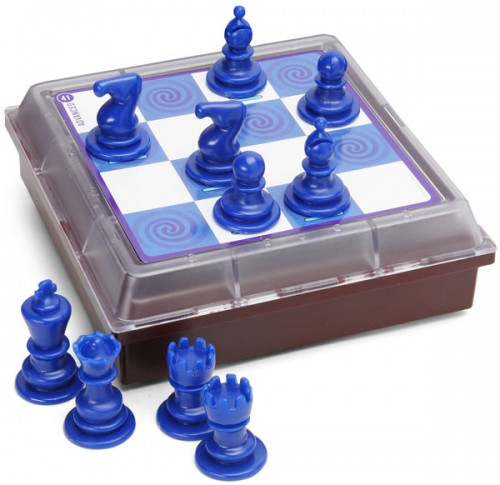
\includegraphics[scale=0.2]{solitaire}
\begin{itemize}

	
	\item pro Zug eine Figur ziehen, um eine andere zu schlagen
	\item 4 x 4- Feld
	\item 10 Figuren : 2 x Bauer, Türme, Springer, Läufer; 1 x König und Dame
	\item Ziel: eine einzige Figur bleibt übrig

\end{itemize}
\end{frame}

\begin{frame}{Fragestellungen}
\begin{itemize}

	\item Welche Startpositionen sind lösbar? (mit variierender Figurenanzahl)
	\item Mögliche Erweiterungen: 
	\begin{itemize}
	\item größeres Spielfeld 
	\item andere Brettform
	\item In wie viel Zügen ist ein Spiel lösbar? 
	\item Wie viele unterschiedliche zum Ziel führende Zugmöglichkeiten gibt es?
	\end{itemize}
\end{itemize}
\end{frame}

\begin{frame}{mögliche Parallelisierung und Größenordnung}
\begin{itemize}

	\item Suchbaum
	\item Ansatz zum Lastausgleich : Teilbäume in Queue verwalten \\(nach Anzahl bereits besuchter Knoten)
	\item Anzahl möglicher Startbelegungen für 4 x 4 mit 2 - 10 Figuren: \\
		ca. $3,5 * 10^{10}$
\end{itemize}
\end{frame}

% Include all the stuff for OS
%\include{betriebssysteme}

% Include all the stuff for Linux
%\include{linuxintro}

\end{document}
